\documentclass[handout]{beamer}
\usepackage[frenchb]{babel}
\usepackage[T1]{fontenc}
\usepackage[utf8]{inputenc}
\usepackage{epstopdf}
% functions to plot
\def\func(#1){(#1)*(1-(#1))}
\hypersetup{colorlinks = true,linkcolor = blue,urlcolor  = blue}

\newcommand{\qGraph}[1]{\begin{center} \includegraphics[width =
\textwidth]{#1}\end{center}}

\newcommand{\mcl}{\mathcal}


\newenvironment{iPar}[1]{\textbf{#1} \begin{itemize}}{\end{itemize}}

\newcommand{\inc}{{inc}}
\newcommand{\cp}{{cmp}}
\newcommand{\bull}{$\bullet\;$} 

\newcommand{\esp}{\mathbf{E}} \newcommand{\ul}[1]{\underline{#1}}
\newcommand{\ol}[1]{\overline{#1}} \newcommand{\ora}[1]{\textbf{#1}}

\newcommand{\mdp}{\medskip \pause}

\title{Mesurer le bien-être}
\author{Microéconmie \\ 20851}
\date{}

\begin{document}

\frame{\titlepage}

\section[Outline]{}
\frame{\tableofcontents}

\section{}

\section{Approche utilitariste}

\begin{frame}\frametitle{Mesurer le bien-être}

\textbf{Approche utilitariste naïve}

\begin{itemize} \item Pour chaque citoyen $i
\in \{1,\ldots,N\}$, trouver la fonction d'utilité $U_i$ qui représente ses préférences sur les paniers trouvés dans $B$
\item Supposons que les citoyens obtiennent les paniers $B_1$, $B_2$, ..., $B_N$

\item Bien-être: $U_1(B_1) + U_2(B_2) + \ldots + U_N(B_N)$
\item Une politique $\mcl P_0$ est meilleure qu'une alternative $\mcl P_1$ si elle procure un plus grand bien-être.
\end{itemize}
\end{frame}
 

\begin{frame}\frametitle{Pourquoi l'utilitarisme naif est inadéquat}
\textbf{Préférences sont ordinales} \begin{itemize}\item Si $U_1$ représente
les préférences du citoyen $1$, $f(U_1)$ représente les mêmes préférences pour n'importe quelle fonction strictement croissance  $f$ \item Par exemple, on aurait pu prendre $2
\times U_1$. \end{itemize}\mdp

\textbf{Implications ne sont pas bien définies} \begin{itemize} \item  $\mcl P_0$ meilleur si $WF = U_1 + U_2$
\item $\mcl P_1$ meilleur si $WF = 2U_1 + U_2$ \item Le bien-être devrait seulement dépendre des préférences et non de $U$. \end{itemize}

\end{frame}

\section{Variation compensatoire}

\begin{frame} \frametitle{Définir le bien-être par les préférences}
\textbf{Utilité indirecte} \begin{itemize}
\item
Politique $\mcl P$ défini une contrainte budgétaire $C_i(\mcl P,I_i)$ pour le citoyen $i$ (où $I_i$ est sa richesse)
\item L'utilité maximale du citoyen $i$ est donné sa contrainte: $$U_i^*(\mcl P,I_i) = \max_{B \in C_i(\mcl P, I_i)} U_i(B)$$
\item Exemple: deux biens $X$ et $Y$. Utilité $U(X,Y) = \log X + \log Y$ \medskip

Politique $\mcl P$: taxe multiplicative $\tau$ sur le prix de
$Y$\mdp

$U_i^*(\mcl P,I) = \max_{X,Y} \log X + \log Y$ \\ s.c. $\quad \quad \quad
p_X  X + p_Y(1 + \tau) Y = I$ \end{itemize}
\end{frame}

\begin{frame}{Variation compensatoire}
  \begin{itemize} \item Politique $\mcl P_0$ est le statut
quo, implémenter la nouvelle politique $\mcl P$ \item Variation compensatoire:  montant $\Delta I^{CV}$  tel que $$U^*(\mcl P_0,I) = U^*(\mcl P,
I - \Delta I^{CV})$$    \item    Montant qu'on peut prendre du consommateur tout en gardant son utilité à son niveau de référence (status quo).  

\item Note: convention de signe tel que  $\Delta I^{CV}>0$ quand changement de politique est \textit{bon} 

 \end{itemize}
 
 \textbf{Exercice A}: Trouvez l'expression de la variation compensatoire pour $\log X + \log Y$ et une taxe $\tau$ sur le bien $Y$. 
\end{frame}

\begin{frame} \frametitle{Propriété fondamentale}

\textbf{Variation compensatoire dépend seulement des préférences:} \begin{itemize} \item $\Delta I^{CV}$ dépend seulement des préférences $$U^*(\mcl P_0,I) = U^*(\mcl P, I - \Delta I^{CV})
\Rightarrow 2 U^*(\mcl P_0,I) = 2  U^*(\mcl P, I- \Delta I^{CV})$$ \item Plus généralement, pour quelconque fonction $f$, $$U^*(\mcl P_0,I) = U^*(\mcl P, I - \Delta I^{CV})
\Rightarrow f[U^*(\mcl P_0,I)] = f[ U^*(\mcl P, I - \Delta I^{CV})]$$\end{itemize}
 
\end{frame}
 
\begin{frame} \frametitle{Cas spécial important}
\textbf{Utilité quasi-linéaire} \begin{itemize} \item Préférence pour un bien $X$ et argent $Y$.
\item Préférences représentées par
 $U(X,Y) = V(X) + Y$
\item Politique référence $\mcl P_0$: allocation $(X_0, Y_0)$
\item Changement $\mcl P$: $(X_1, Y_1)$. \end{itemize} \mdp

\end{frame}

\begin{frame} \frametitle{Variation compensatoire}

$\Delta I^{CV}$ tel que 
\begin{eqnarray*}
U(X_0,Y_0) &=& U(X_1, Y_1- \Delta I^{CV}) \\
V(X_0) + Y_0 &=& V(X_1) + Y_1 - \Delta I^{CV} \\
\Delta I^{CV} &=& V(X_1) + Y_1 - V(X_0) - Y_0 \\
\Delta I^{CV} &=& U(X_1,Y_1) - U(X_0,Y_0)
\end{eqnarray*}

Variation compensatoire est égale au changement d'utilité 
 \end{frame}

\section{Surplus du consommateur}

\begin{frame} \frametitle{Surplus du consommateur pour achats}

\textbf{Supposons utilité quasi-linéaire} \begin{itemize} \item Bien $X$
et argent $M$. $U(X,M) = V(X) + Y$ \item Supposons $V$ concave ($dV/dX$
décroissant en $X$) 
\item Considérons   $\mcl P_0$ ne peut acheter $X$  
\item Alternative $\mcl P$ permet d'acheter $X$ au prix $p_X$ \\\mdp
$\max_{X,Y} U(X,Y) \quad s.c. \quad p_X X + Y = I$

\item Équivalent à $\max_{X} V(X) + I - p_X X$
CPO: $ \frac{dV}{dX}_{|X^*} =  p_X$\\ Donne la demande $X^*(p_X)$ \end{itemize}\mdp

\end{frame}

\begin{frame}{Surplus du consommateur}

Variation compensatoire de $\mcl P_0$ à $\mcl P$ est le surplus du consommateur. 

\begin{eqnarray*}
\Delta I^{CV} &=& V[X^*(p)] + I - pX^*(p) - [V(0) + I] \\
&=& V[X^*(p)] - V(0) - p X^*(p)
\end{eqnarray*}

\end{frame}

\begin{frame} \frametitle{Perte de bien-être venant d'une taxe}
\textbf{Tax: passage de $p_X = p+t$    à $p_X = p$  .} \begin{itemize}
\item Nouvelle consommation $X^*(p) > X^*(p+t)$ \item Revenu de la taxe $T
= t\times X^*(p+t)$ \item Variation compensatoire 
\begin{eqnarray*}
U[X^*(p), I - pX^*(p)] - U[X^*(p+t), I - (p+t) X^*(p+t)]
\end{eqnarray*}
\end{itemize}\mdp


\textbf{Propriété} \begin{itemize} \item $\Delta I^{CV} > T$: disposition à payer pour éviter taxe plus élevé que revenu généré par gouvernement \item Perte de bien-être associé à la taxe $= \Delta I^{CV} - T$ \end{itemize}



\end{frame}

\begin{frame} \frametitle{Perte de bien-être venant d'une taxe}

\textbf{Exercice B}: Si $V(X) = 10 X - \frac{1}{2}X^2$, trouvez la perte de bien-être associé à une taxe $t$ sur le bien $x$. 
\end{frame}

\section{Application: Valeur de la qualité de l'air}
\begin{frame}{Application: Valeur de la qualité de l'air }
\begin{iPar}{Question de politique}
\item Aucun marché pour l'air (de qualité), doit être protégé (offert) par gouvernement.
\item Le Clean Air Act 1977, gouvernement met en place des mesures pour réduire la pollution.
\item E.g. 1990: Contrôle d'emission des véhicules
\item Règlementation est coûteuse, payé indirectement par des taxes, des prix plus élevés
\item Question: est-ce que ces mesures augmentent le bien-être?
\end{iPar}\mdp

\begin{iPar}{Comment répondre à cette question}
\item Considérons changement de politique $\mcl P_0$: aucun contrôle, aucun coût, à $\mcl P$: contrôle de pollution à un coût
\item Variation compensatoire >0 (convention de signe), les citoyens accordent une valeur à cette politique.
\end{iPar}
\end{frame}


\begin{frame}{Comment faire?}
\begin{iPar}{Étape 1: Estimer les préférences des gens}
\item Trouver une situation ou les citoyens font un arbitrage entre la pollution et la richesse (consommation de biens).
\item E.g. Acheter une maison. Grande variation à l'intérieur d'une ville.\mdp
\item \textbf{Contrôlant pour d'autres facteurs}, utiliser des données de transactions immobilières pour déterminer la valeur accordée à la qualité de l'air
\item e.g. Définir X = mesure de qualité de l'air \\ (e.g. concentration de particules) \pause

Estimer $U(X, Y) = V(X) + Y = \alpha X + \beta X^2 +Y$

\end{iPar}\mdp 

\end{frame}

\begin{frame}{Évaluation de la politique}

\begin{iPar}{Calcul de la variation compensatoire}
\item Gouvernement dépense $X_{GOV}$. Vient à un coût $c\times X_{GOV}$ aux contribuables (utiliser la perte de bien-être par dollar de revenu de taxe).
\item Considérons le changement de politique de   $(0,0)$ à  $(X_{GOV}, - c \times X_{GOV})$
\item Surplus du consommateur est la variation compensatoire $\Delta I^{CV} =  V(X_{GOV}) - c X_{GOV} - V(0)$.
\end{iPar}\mdp

\begin{iPar}{Pollution optimale}
\item La valeur optimale de la pollution est celle qui maximise $X^*$ s.c \mdp
La CPO est
$$\frac{dV}{d X}_{|X^*} = c$$
\end{iPar}

\end{frame}



\begin{frame}{Évaluation de la valeur accordée à la qualité de l'air}
\begin{figure}
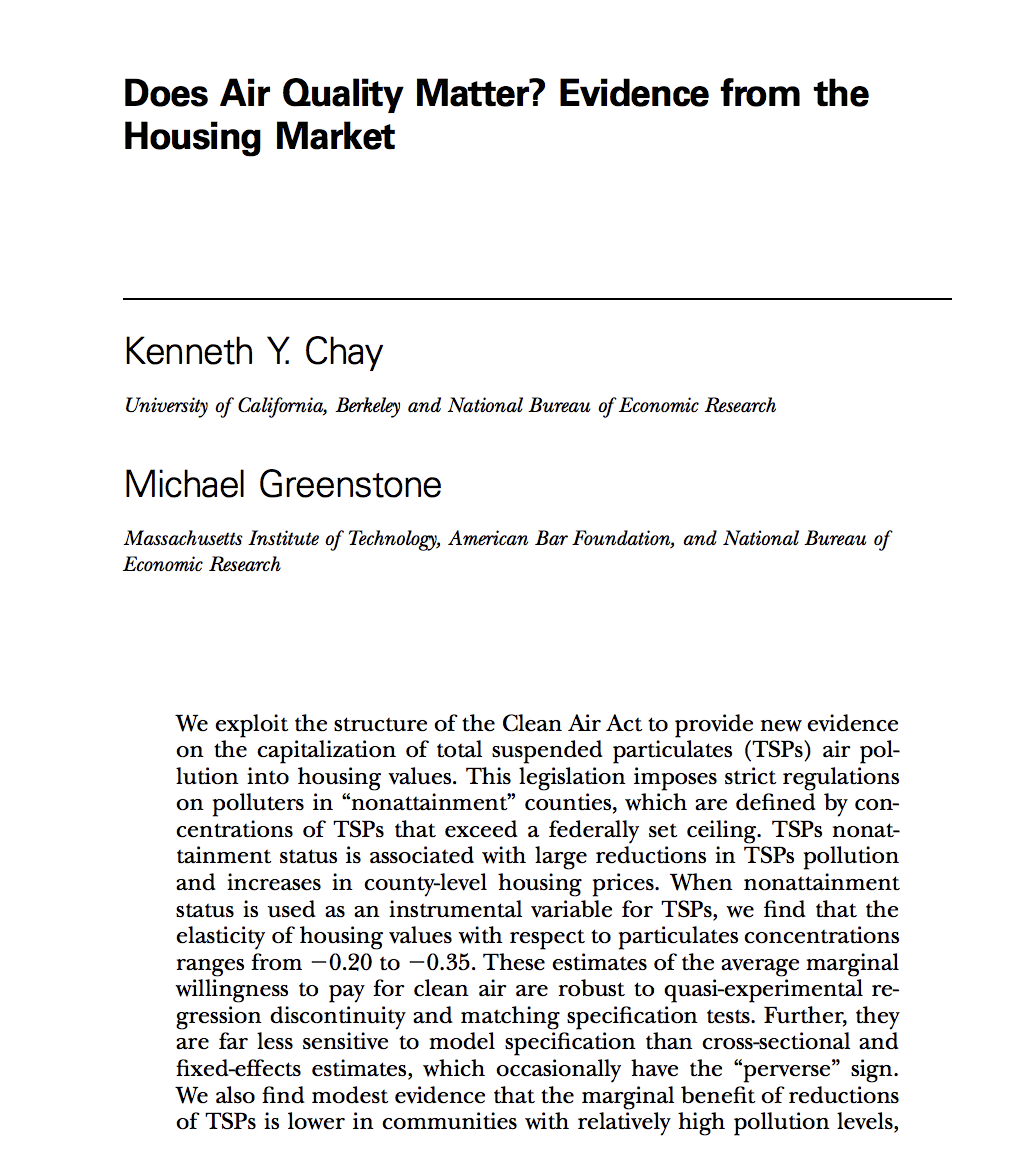
\includegraphics[scale=0.3]{chay.png}
\caption{\href{https://www.jstor.org/stable/10.1086/427462}{Chay et Greenstone (2005), Journal of Political Economy}}
\end{figure}
\end{frame}

\begin{frame}{Exemple: Pollution sonore}

\begin{itemize}
	\item L'élasticité du prix des maisons à la pollution sonore est de -0.2
	\item Le gouvernement considère de diminuer la pollution sonore de 10\% en bordure d'une autoroute. 
	\item Les ingénieurs nous disent que de construire un mur anti-bruit va coûter 1000\$ par propriétaire touché
	\item Cette dépense serait financée par une taxe spéciale qui crée une perte de bien-être de 43 cent par dollar de taxe. 
\end{itemize}
	
\textbf{Exercice C}: Cette politique augmente-elle le bien-être des citoyens touchés?
\end{frame}

\section{Mesurer le bonheur}

\begin{frame}{Mesurer directement le bien-être}

\begin{itemize}
\item Approche de variation compensatoire du à \href{https://fr.wikipedia.org/wiki/John_Hicks}{John Hicks}
\item Pourquoi ne pas demander aux gens s'ils sont heureux?
\item Projet de la Nouvelle-Zélande
\item \href{https://fr.wikipedia.org/wiki/Richard_Easterlin}{Richard Easterlin} a popularisé ceci (relation entre bonheur et revenu par habitant presque nulle)
\end{itemize}


\end{frame}

\begin{frame}{Le Paradoxe d'Easterlin}

\begin{figure}
\centering
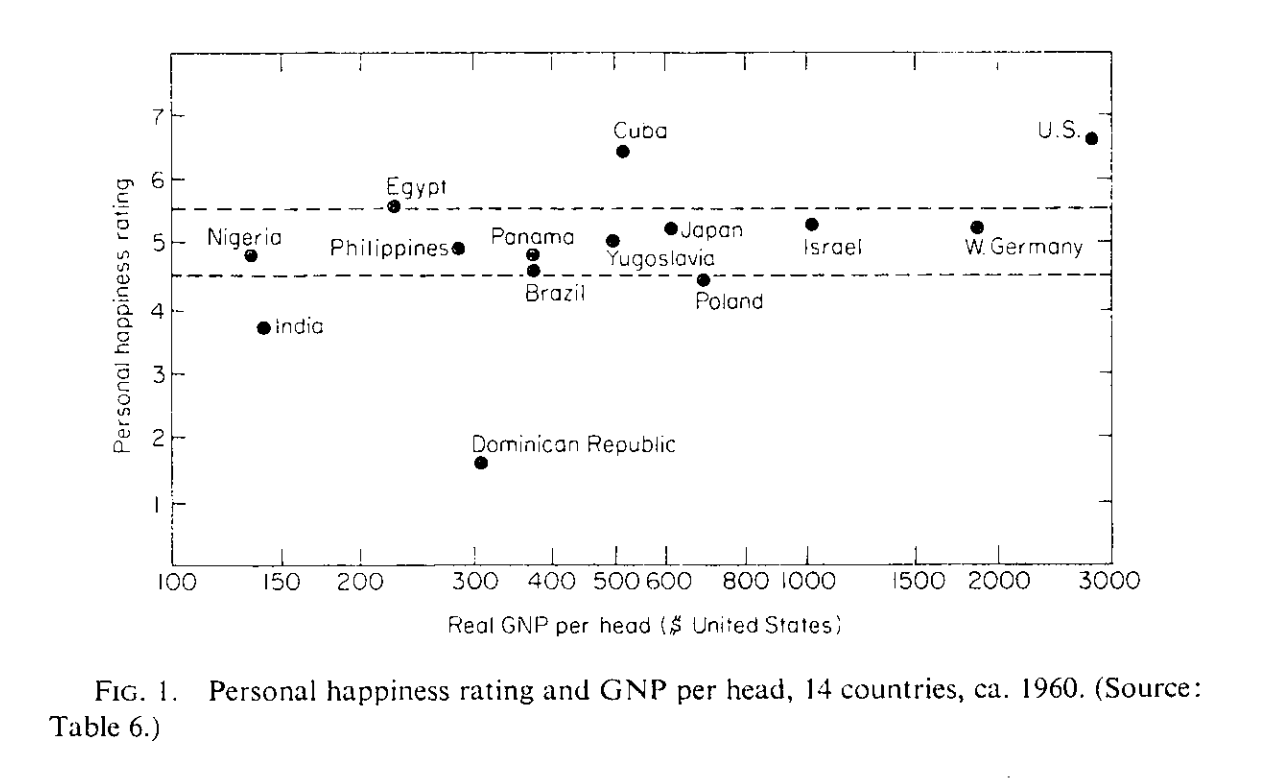
\includegraphics[scale=0.3]{easterlin.png}
\caption{\href{http://graphics8.nytimes.com/images/2008/04/16/business/Easterlin1974.pdf}{Easterlin (1974)}}
\end{figure}

\end{frame}


\begin{frame}{Y-a-t-il un paradoxe?}

\begin{figure}
\centering
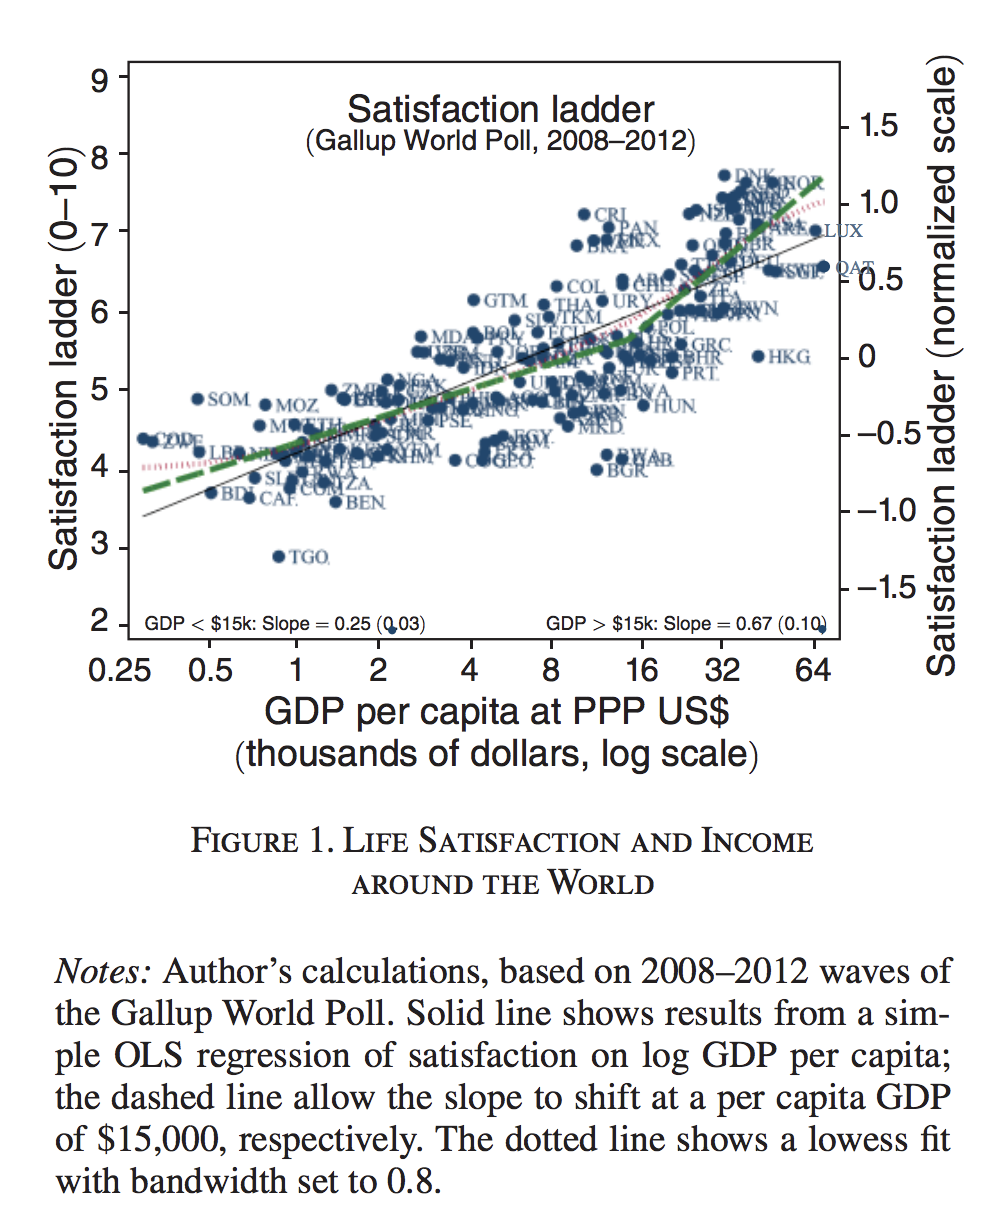
\includegraphics[scale=0.3]{wolfers.png}
\caption{\href{http://users.nber.org/~jwolfers/papers/Satiation(AER).pdf}{Stevenson and Wolfers (2013), AER: Papers and Proceedings}
}
\end{figure}

\end{frame}

\begin{frame}{Utiliser les mesures de bonheur pour évaluer les politiques}

\begin{itemize}
\item Pourquoi ne pas regarder impact d'une politique sur le bonheur?
\item Avantages: évaluation directe sans modèle, prend toutes les dimensions en compte
\item Désavantages: Les gens ont des échelles pour rapporter bonheur qui sont différentes, le choix de la question peut être important, différents effets psychologiques
\end{itemize}

On voit peu d'analyses qui incluent ces mesures. Mais beaucoup d'intérêt chez les gouvernements. 
\end{frame}

\end{document}




